\RequirePackage{lineno}
\documentclass[12pt]{article}
\usepackage[final]{graphicx}
\usepackage{ucs,multicol,natbib,ifdraft,mathtools,xfrac,float,array}
\usepackage[hidelinks]{hyperref}
\usepackage[utf8x]{inputenc}
\usepackage[T1]{fontenc}
\usepackage[romanian]{babel}
\usepackage[a4paper,margin=2cm]{geometry}
\usepackage[printonlyused,withpage]{acronym}
\usepackage[usenames]{color}
\usepackage[obeyDraft,colorinlistoftodos]{todonotes}

\floatstyle{boxed}
\restylefloat{figure}
\setlength{\columnsep}{25pt}

\graphicspath{ {./img/} }
\DeclareGraphicsExtensions{.pdf,.png,.jpg}

\presetkeys{todonotes}{inline}{}

\bibpunct{(}{)}{;}{a}{,}{,}
 
\makeatletter
\def\closeopenmulticols{%
   \def\@tempa{multicols}%
   \ifx\@tempa\@currenvir
      \end{multicols}%
  \fi 
}

\makeatother
\newcommand\Section[1]{%
 \closeopenmulticols
 \ifdraft{\begin{multicols}{2}[\section{#1}]}{\section{#1}}
}


% close last open multicols
\AtEndDocument{ \closeopenmulticols}

\title{Studiu observațional asupra tratamentului incontinenței urinare de efort la pacientele din ambulator}
\author{Dr.~Andrei~Manu-Marin,~medic~primar~urologie\\Gnosis-EvoMed, str.~Suvenir,~nr.~10,~sect.~2,~București}
\date{\todo{data studiu}}

\begin{document}

%\ifdraft{}{\fontsize{6mm}{9mm}\selectfont}

\maketitle\ifdraft{\linenumbers}{ }\todototoc\listoftodos

\begin{abstract}
\ac{IU} este definită ca orice pierdere involuntară a urinei. \ac{IU} face parte din categoria de simptome ale tractului urinar inferior (prescurtare: \ac{LUTS}) care includ dificultăți atât legate de stocarea urinei cât și de eliminarea ei, \ac{IU} fiind în categoria simptome de stocare. Tratamentul aplicat acestor pacienți îmbunătățește semnificativ toate valorile urmărite, atât pe cele subiective cât și pe cele obiective, reduce cu 87\% ($\approx2\sigma$) numărul de episoade de incontinență și mărește cu 50\% ($\approx2\sigma$) forța musculaturii perineale. Aceste efecte sunt robuste indiferent dacă pacienții suferă de \acf{IUE} sau \acf{IUI}.
\end{abstract}
  
\Section{Introducere}
\ac{IU} este definită ca orice pierdere involuntară a urinei. \ac{IU} face parte din categoria de simptome ale tractului urinar inferior (prescurtat, \ac{LUTS}) care includ dificultăți atât legate de stocarea urinei cât și de eliminarea ei, \ac{IU} fiind in categoria simptome de stocare. \ac{IU} poate fi caracterizată în plus prin datele obținute în urma anamnezei și a contextului simptomelor descrise de pacient.  

\ac{IUI} se definește ca pierderea de urină precedată de senzatia intensă de a urina, numită imperiozitate. \ac{IUE} se definește ca eliminarea involuntară de urină asociată cu anumite activități fizice (de ex. strănut și tuse). \ac{IUM} include caracteristici atât ale \ac{IUI} cât și ale \ac{IUE}. 

Incontinenţa este denumită de efort atunci cînd apare strict în cadrul unor eforturi fizice. Aceasta poate fi uşoară cînd apare uneori în timpul unui efort sportiv (fitness). Este considerată medie cînd apare la eforturi obişnuite: ridicat de pe scaun, rîs, strănut, tuse, etc. Este considerată gravă cînd este permanentă. Aceasta este aprecierea medicală a pierderii de urină însă, importantă rămîne aprecierea pe care o are pacienta asupra gravităţii acestei probleme.
Studiile clinice \todo{Care?} au demonstrat că pierderea de urină apare mai frecvent la sexul feminin deoarece aparatul sfincterian al vezicii urinare este mai slab, principalul element care menţine continenţa la femei fiind musculatura perineală. Sarcina şi naşterea pot altera frecvent inervaţia şi integritatea pelvi-perineală. Urmarea este un control mai dificil al continenţei urinare şi fecale. 

Incontinenta urinara este un simptom care afecteaza calitatea vietii pacientelor, fapt dovedit de studii populationale. Acestea au evidentiat grade de afectare a calitatii vietii la pacientele cu \ac{IU} asemanatoatre cu cele care au suferit un infarct miocardic. Prevalenta \ac{IU} a fost apreciata de diverse studii populationale ca fiind situata intre 10 si 50\% \todo{Referinte?}. 
In Romania, incontinenta urinara reprezinta o preocupare mai veche a mea, primul pas facut in acest domeniu fiind un studiu efectuat in perioada octombrie-decembrie 2001, completat de un esantion ($n=674$) reprezentativ pentru populatia de femei active profesional.
Obiectivul studiului a fost de a aprecia prevalenta incontinentei urinare la femeile tinere si adulte, active profesional cat si asocierea incontinentei urinare cu factorii de risc: varsta, efort fizic, nasteri, interventii chirurgicale, boli cronice, infectii urinare joase cit si prevalenta cistitei la lotul de femei studiat.
Dintre participante, 10,8\% au afirmat incontinenta. Din acestea 67,6\% prezinta incontinenta de efort, 16,9\% incontinenta prin imperiozitate, 15,5\% incontinenta mixta. 
Dintre femeile cu \ac{IU} 97\% s-au declarat nemultumite de conditia lor. Doar 25\% au consultat medicul pentru IU si doar 18\% au urmat un tratament. 
Dintre factorii de risc evaluati varsta, efortul fizic in activitatea profesionala, nasterile in antecedente si bolile ce se insotesc de tuse cronica se asociaza semnificativ cu riscul de IU. 
Din punct de vedere al cistitelor, 62,9\% au declarat ca au avut cel putin un episod de polachiurie cu disurie si senzatie de arsura uretrala.
Doar 16\% din aceste femei au prezentat mai mult de un episod de cistita pe an ; 70\% au consultat un medic pentru aceste simptome. 
Analiza statistica nu a demonstrat nici o corelatie intre frecventa de aparitie a cistitei si efortul fizic, sau numarul de nastrei, sau incontinenta urinara. 
Principala concluzie a fost aceea ca toate femeile cu incontinenta urinara, chiar si cele care pierd ocazional, au declarat ca se simt groaznic, cu toate acestea doar 25\% au consultat un medic. \citep{Manu04}.

Pacienților care prezintă semne și simptome de IU li se recomandă efectuarea unei evaluări medicale complete pentru a elimina cauze nonfunctionale ce ar putea produce tulburarile urinare, tumori, infectii, diabet. Importanța unui diagnostic corect nu este exagerată. 
Pentru elaborarea unui plan adecvat de tratament este necesară o analiză completă a istoricului pacientului, inclusiv a comorbidităților si abordarea si a acestora din urma, de rezolvarea lor (hemoroizi, hernie de disc intervertebral, constipatie, hiperglicemie, obezitate, etc) depinzind mare parte din succesul tratamentului.

Tratamentul IU include metode conservative, de reeducare/refacere a echilibrului vezico sfincterian si metode chirurgicale ireversibile, slingul suburetral, introdus transobturator (\ac{TOT}) sau suprapubian (\ac{TVT}) fiind in prezent operatia cea mai frecvent efectuata. 
Pînă recent medicii ofereau acestor paciente doar soluţii chirurgicale, cel mai frecvent operaţii de fixare sau ridicare a organelor genitale sau a vezicii urinare. Metodele chirurgicale au evoluat în sensul apariţiei unor intervenţii cu spitalizare minimă (sling, TVT), sau efectuării laparoscopice a unor intervenţii chirurgicale clasice (Burch) \todo{Cite adevarat}. 
Acestea oferă rezultate favorabile variabile, astfel încît 70-90\% dintre paciente nu mai pierd urină în primul an după operaţie. Aceste rezultate, însă,  se alterează cu fiecare an trecut de la operaţie. 

Acest fapt a dus la căutarea unor soluţii mai eficiente, mai simple şi mai ieftine de rezolvare a pierderilor de urină. În acelaşi timp, au fost studiate şi introduse metode mai puţin agresive, mai comode pentru pacientă. 
Studiile \todo{Care?} au arătat că peste 60\% dintre pacientele care sunt tratate conform unor metode de antrenament muscular sub control medical, însoţite sau nu de stimulare electrică isi îmbunătăţesc situaţia si nu mai au nevoie de operaţie. Întrucât nu se poate obține cura completă a incontinenței prin nici o metodă, ghidurile terapeutice din Europa și America \todo{Ref?} recomandă tratamentul conservator de refacere a echilibrului vezico sfincterian ca prima linie de tratament in IUE, iar optiunea chirurgicala, slingul suburetral, ca a doua linie de tratament in IUE.

%%%%    
\Section{Metode}

\subsection{Protocolul clinic}
  Studiul este unul observațional care evaluează răspunsul unui grup de pacienți tratat ambulatoriu pe o perioada de 12 săptămâni de tratament. Au fost înrolați 50 pacienți de ambele sexe(F=31,M=19) pe o perioada de 8 săptămâni ($\pm$ 4 săptămâni). Criteriile de includere au fost:
  \begin{itemize}
    \item Incontinență urinară timp de cel puțin trei luni
    \item Bărbați și femei adulți tratați în ambulator
    \item Mai mult de 1 episod de IU pe zi conform jurnalului micțiunilor de 2 zile
    \item IU dovedită în timpul testelor urodinamice
   \end{itemize}
 
 Criteriile de excludere au fost:
  \begin{itemize}
    \item Pierdere continuă de urină.
    \item Sarcină sau planificare a unei sarcini în interval de 1 an.
    \item Infecție activă a tractului urinar.
    \item Retenție urinară.
    \item Antecedente de tumori ale vezicii urinare, intervenție chirurgicală împotriva cancerului la nivel pelvin (amputație de rect, histerectomie radicală)
    \item Iradiere pelvină
    \item Sub medicație curentă pentru incontinență.
    \item Condiție neurologică care afectează funcția vezicii urinare.
    \item Deficiență mintală 
    \item Intervenție chirurgicală anterioară pentru IU
    \item Intervenție chirurgicală anterioară pentru patologia prostatei 
   \end{itemize}
  Pacienții incluși au efectuat proceduri de recuperare și stimulare periferică timp de 8 săptămâni constând în 3 sesiuni de \ac{SEP} pe săptămână pentru 8 săptămâni și 3 sesiuni de fizioterapie pe săptămână pentru 4 săptămâni începând din săptămâna 5. Ulterior, pacienții au fost instruiți sa facă exerciții fizice acasă, fără supraveghere timp de 4 săptămâni. O vizită de evaluare și urmărire a fost efectuata la 6 luni de la includerea în studiu.
  
  Pacienților le-au fost administrate la începutul și sfârșitul tratamentului 4 chestionare care cuprind evaluări subiective folosind o scală psihometrică Likert:
  \begin{itemize}
    \item \ac{CEII} -- sunt enumerate 7 activități uzuale și se cere pacienților să evalueze pe o scară discretă de la 0 la 3 (valori mai mari indică impact negativ mai important), care este impactul pierderilor de urină. Este înregistrată suma evaluărilor.
    \item \ac{CVDSU} -- evaluează pe o scară discretă de la 0 la 7, impresia asupra calității vieții viitoare condiționată de prezența pierderilor de urină. Valori mai mari reprezintă o calitate a vieții inferioară.
    \item \ac{VAS} -- evaluează pe o scară discretă de la 0 la 10, impresia asupra calității vieții actuale condiționată de prezența pierderilor de urină. Valori mai mari reprezintă o calitate a vieții inferioară.
    \item \ac{IGPI} -- evaluează pe o scară discretă de la 0 la 7, impresia pacienților asupra efectului tratamentului. 1 reprezintă efect pozitiv maxim, 4 reprezintă nici un efect, 7 reprezintă efect negativ maxim.
  \end{itemize}
  De asemenea, următorii parametrii obiectivi au fost înregistrați folosind chestionare administrate la începutul și sfârșitul tratamentului pentru a putea urmării eficacitatea acestuia:
  \begin{itemize}
    \item I2D -- înregistrează numărul de episoade de incontinență din ultimele 2 zile premergătoare completării chestionarului. 
    \item \ac{FEFMP} -- înregistrează calitatea contracției musculaturii pelvine pe o scara discreta de la 1 la 5 cu valori mai mari reprezentând o contracție puternică. 
    \item \ac{USS} -- înregistrează numărul de vizite la medicul de familie și medicul specialist urolog/ginecolog în ultimele 3 luni anterioare administrării chestionarului, legate de prezența pierderilor de urină.
  \end{itemize}

\subsection{Metode statistice}
  Pentru a analiza datele au fost folosite mai multe metode matematice bazate atât pe abordarea asa zis fregvenționistă cât și pe cea bayesiana. Datele au fost analizate folosind mediul de dezvoltare numit R (http://www.r-project.org/). Mai jos sunt prezentate pe scurt câteva dintre metode împreună cu referințe bibliografice pentru mai multe detalii.

\subsubsection{Testul Wilcoxon}
 \textbf{Testul Wilcoxon} este un test non-parametric pentru a testa ipoteza statistică de egalitate a primului moment pentru doua populații care se folosește atunci când distribuția celor 2 populații nu este normală (alternativa pentru populații normale este Testul Student t, sau Testul Z). 
 Populațiile trebuie sa îndeplinească următoarele condiții:
 \begin{itemize}
  \item Datele examinate provin din aceeași populație
  \item Datele sunt aleatoare, independente și identic distribuite
  \item Datele sunt reprezentate prin numere întregi sau reale
  \item Distribuția este simetrică în jurul valorii medianei.
 \end{itemize}
  Testul împerechează datele din cele 2 populații $(x_{2,i},x_{1,i})$, elimina perechile de valori identice, și le sortează în ordinea crescătoare a diferenței absolute $|x_{2,i}-x_{1,i}|$ cu $R_i=1, ..., N_r$ semnificând rangul perechii $(x_{2,i},x_{1,i})$ după ordonare. 
  Ulterior se calculează statistica $W = |\sum_{i=1}^{N_r} [sgn(x_{2,i} - x_{1,i}) \cdot R_i]| $ și un scor $p = \frac{W - 0.5}{\sigma_W}, \sigma_W = \sqrt{\frac{N_r(N_r + 1)(2N_r + 1)}{6}}$. 
  Dacă scorul este mai mare decât un prag convențional ales $0.05$ atunci ipoteza $H_0$ de egalitate a primului moment este rejectată. 
  Pentru detalii vezi \citep{wilcoxon45,siegel56}.

\subsubsection{Testul Fisher}
 \label{testFisher}
 \textbf{Testul Fisher} este un test exact în sensul că poate calcula exact deviația de la ipoteza nulă pentru că ia în calcul toate posibilitățile de combinare a factorilor, care se folosește pentru tabelele de contingență ale datelor categoriale în cazul în care numărul de categorii este mic (pentru multe categorii calculul este complicat pentru că apar probleme numerice legate de lucru cu valori foarte mari generate de distribuția hipergeometrică și funcția $\Gamma$). Statistica folosită este $p = \frac{ \displaystyle{{a+b}\choose{a}} \displaystyle{{c+d}\choose{c}} }{ \displaystyle{{n}\choose{a+c}} } = \frac{(a+b)!~(c+d)!~(a+c)!~(b+d)!}{a!~~b!~~c!~~d!~~n!}$ care reprezintă probabilitatea de a obține un tabel de contingență cu valorile $a, b, c, d, n=a+b+c+d$ din setul tuturor tabelelor posibile. Alternativa testului Fisher este testul $\chi^2$ (chi pătrat). Pentru detalii vezi \citep{fisher1922interpretation}.

\subsubsection{Testul Kolmogorov–Smirnov}
 \label{testKS}
 \textbf{Testul Kolmogorov–Smirnov} este un test non-parametric pentru ipoteza statistică de proveniență din aceeași distribuție continuă și unidimensională pentru doua eșantioane care se folosește atunci când distribuția nu este normală (teste mai puternice pentru a determina normalitatea datelor sunt  Shapiro–Wilk sau Anderson–Darling \citep{Stephens74} ). 
 Plecând de la distribuția empirică descrisă de funcția $F_n(x)={1 \over n}\sum_{i=1}^n I_{X_i\leq x}$ unde $X_i$ sunt variabile independente și identic distribuite, iar $I_{X_i\leq x}$ este funcția indicator egală cu $1$ dacă $X_i\leq x$ și cu $0$ în rest, se calculează statistica Kolmogorov–Smirnov $D_{n,n'}=\sup_x |F_{1,n}(x)-F_{2,n'}(x)|$ pentru o fiecare distribuție empirică $F_{i,n}(x)$ dată. 
 Teorema lui Kolmogorov arată că ipoteza nulă este rejectată cu o probabilitate p dacă $D_{n,n'}\sqrt{\frac{n n'}{n + n'}}>K_\alpha$ unde $K_\alpha$ este obținut din $Pr(K\leq K_\alpha)=1-\alpha$ cu $Pr(K\leq x)$ fiind distribuția cumulativă de probabilitate dată de $Pr(K\leq x)=1-2\sum_{k=1}^\infty (-1)^{k-1} e^{-2k^2 x^2}=\frac{\sqrt{2\pi}}{x}\sum_{k=1}^\infty e^{-(2k-1)^2\pi^2/(8x^2)}$. 
 Pentru detalii vezi \citep{stuart99}.

\subsubsection{Testul Student t}
 \label{testT}
 \textbf{Testul Student t} sau \textbf{testul t} este un test parametric pentru ipoteza statistică nulă de egalitate a mediei intre 2 eșantioane ($X_1,X_2$) sau intre media unui eșantion și o valoare specificată. Statistica testată este $t = \frac{\bar {X}_1 - \bar{X}_2}{S_{X_1X_2} \cdot \sqrt{\frac{1}{n_1}+\frac{1}{n_2}}}$ cu $ S_{X_1X_2} = \sqrt{\frac{(n_1-1)S_{X_1}^2+(n_2-1)S_{X_2}^2}{n_1+n_2-2}}.$ și $S_{X_1},S_{X_1}$ sunt deviațiile standard, iar $\bar {X}_1,\bar{X}_2$ sunt mediile ale eșantioanelor $X_1,X_2$.
 Eșantioanele trebuie sa îndeplinească următoarele condiții:
 \begin{itemize}
  \item Provin din aceeași populație cu o distribuție normală
  \item Datele sunt aleatoare, independente și identic distribuite
  \item Deviația standard $S^2$ a eșantioanelor are o distribuție de tipul $\chi^2$ (chi pătrat)
 \end{itemize}
 Testul t este robust la variațiile datelor de la normalitate dar se vor urmări câteva recomandări înainte de aplicarea lui:
 \begin{itemize}
  \item Să se verifice folosind metoda grafică dacă datele urmăresc o distribuție de tip ``cocoașă``
  \item Dacă dispersia $var(x)$ celor 2 eșantioane nu este egală (testabilă folosind testul F, Levene, Bartlett sau cu un grafic Q-Q) trebuie aplicată corecția Welch care modifică statistica t în $t = {\overline{X}_1 - \overline{X}_2 \over s_{\overline{X}_1 - \overline{X}_2}}$ cu $s_{\overline{X}_1 - \overline{X}_2} = \sqrt{{s_1^2 \over n_1} + {s_2^2  \over n_2}}$
  \item Comparat cu testul Wilcoxon, testul t este potrivit pentru analiza datelor colectate folosind scale Likert deoarece are rezultate comparabile cu acesta în cazurile uzuale și chiar superioare dacă premizele testului Wilcoxon nu sunt îndeplinite: distribuția este multi-modală sau puternic deplasată spre extreme. Vezi \citep{clason1994analyzing,deWinter12}.
 \end{itemize}
 Pentru detalii vezi \citep{welch1947generalisation}.
  
%%%%    
\Section{Rezultate}
\subsection{Populația}
 \label{rezPop}
  Un număr de 50 de pacienți au fost observați. Dintre aceștia 62\% (N=31) sunt de sex feminin, iar 38\% (N=19) sunt de sex masculin (proporția sexelor în grupa populației urbane cu vârste cuprinse între 27 și 83 ani la nivel național conform \citep{insee2011} este de 47\% M și 53\% F). 25 dintre aceștia suferă de \ac{IUE} și 25 de \ac{IUI}.
  Vârsta pacienților de sex feminin este distribuită normal în jurul mediei de 50 de ani și 7 luni ($\sigma=14.3,min=27,max=77$), iar cea a pacienților de sex masculin este o combinație de distribuții normale centrate în jurul mediilor de 46,  respectiv 75 ani ($\sigma_{1}=12.3 , \sigma_{2}=9.2,min=30,max=83$).
  Pentru a evalua reprezentativitatea eșantionului relativ la distribuția vârstelor în cadrul populației din Romania am apelat la datele oficiale din \citep{insee2011} care detaliază numărul de cetățeni romani pe sexe și categorie urban/rural pentru fiecare vârstă la data de 1 iulie 2010. 
  Analiza statistică s-a efectuat folosind testul Wilcoxon, iar concluzia este că atât eșantionul de sex feminin ($p=0.9964$) cât și cel de sex masculin($p=0.9967$) corespund cu distribuția generală în populațiă urbană a României.
  %
  \begin{figure}[H]
   \centering
   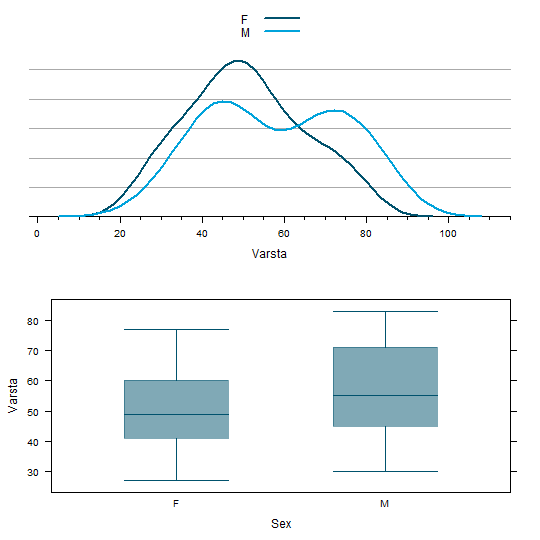
\includegraphics[width=0.8\linewidth]{incoVarstaSex}
   \caption{Distribuția sexelor participanților la studiu}
   \label{fig:Distributia sexelor participantilor la studiu}
  \end{figure}
  %
  Din punct de vedere al greutății am evaluat indicatorul \ac{BMI} conform cu pragurile recomandate de \citep{whobmi06}. 
  Astfel, pentru pacienții de sex feminin avem 13 persoane cu greutate normală ($BMI<25.0$, NOR), 16 supraponderale ($25.0 \geq BMI <30.0$, OVR) și 2 obeze($BMI \geq 30.0$, OBE). 
  Pentru pacienții de sex masculin avem 3 persoane cu greutate normală, 12 supraponderale și 4 obeze.   
  %
  \begin{table}[H]
   \centering
   \begin{tabular}{ |l|l|l|l| }
    \hline
    Sex & NOR & OVR & OBE \\ \hline
    F & 13 & 16 & 2 \\ \hline
    M & 3 &  12 & 4 \\ \hline
   \end{tabular}
   \caption{Numărul de persoane din fiecare categorie \ac{BMI} pe sexe}
   \label{tab:BMIgSex}
  \end{table}
  %
  \begin{figure}[H]
    \centering
    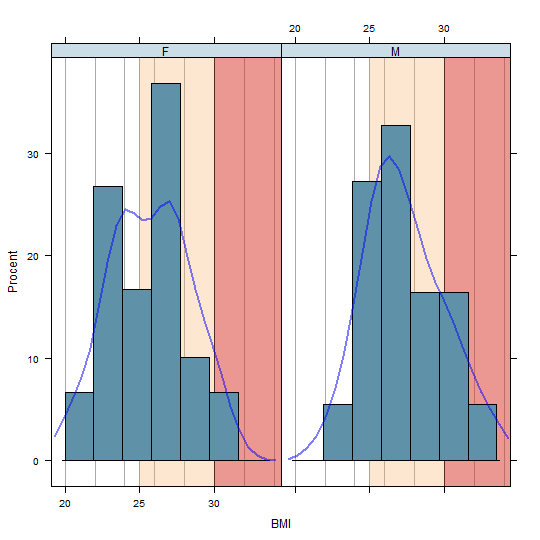
\includegraphics[width=0.8\linewidth]{incobmiDens}
    \caption{Distribuția \ac{BMI} pe sexe. Zona mai deschisă marchează persoanele supraponderale și cea mai închisă pe cele obeze}
    \label{fig:incobmiDens}
  \end{figure}
  %
  Distribuția \ac{BMI} pe grupa de vârstă și pe sexe a fost evaluată la nivel național conform \citep{EHIS09}, care oferă informații detaliate despre incidenta problemelor de nutriție în rândul țărilor membre ale Uniunii Europene. 
  Din cauza eșantionului foarte mic, nu se poate trage concluzia că populația studiată provine dintr-un eșantion aleator la nivel național, dar examinând graficul din Figura~\ref{fig:incoBMIvsEHIS-OOB} se poate observa (cu excepția unor situații particulare - de exemplu toate persoanele de sex masculin din grupa de vârstă 25-44 ani sunt supraponderale sau obeze) că valorile procentelor urmăresc distribuția națională.
  Pentru a testa dacă eșantioanele provin din aceeași distribuție comună am folosit testul \ac{KS}, care a dat o probabilitate de 60\% pentru persoanele de sex feminin și de doar 12.4\% pentru persoanele de sex masculin indicând că datele nu sunt suficiente pentru a susține în mod concludent reprezentativitatea eșantionului sau că există un bias de selecție a pacienților în funcție de \ac{BMI}.
  %
  \begin{figure}[H]
    \centering
    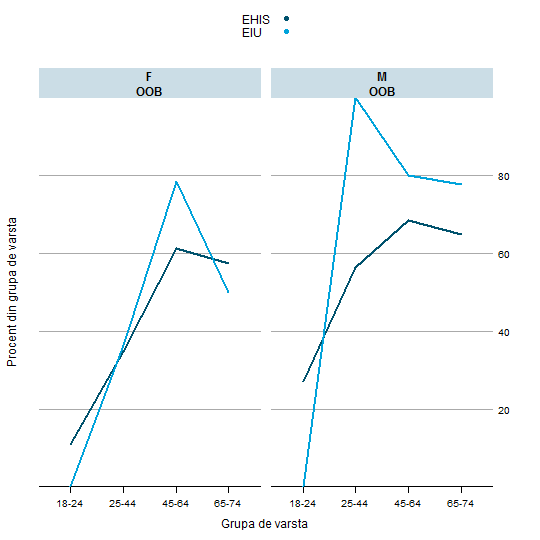
\includegraphics[width=0.8\linewidth]{incoBMIvsEHIS-OOB}
    \caption{Distribuția procentului de persoane obeze în populația studiata (EIU) și în populația generala (EHIS) }
    \label{fig:incoBMIvsEHIS-OOB}
  \end{figure}
  %
  \closeopenmulticols\begin{table}[H]
    \centering
    \begin{tabular}{ |l|l|l|l|l| }
      \hline
      Grupa de vârstă & Sex & Categorie BMI & Număr persoane & Procent \\ \hline
      25-44 & F & NOR & 7  & 63.6 \\ \hline
      25-44 & F & OVR & 3  & 27.3 \\ \hline
      25-44 & F & OBE & 1  &  9.1 \\ \hline
      25-44 & M & NOR & 0  &  0.0 \\ \hline
      25-44 & M & OVR & 4  & 80.0 \\ \hline
      25-44 & M & OBE & 1  & 20.0 \\ \hline
      45-64 & F & NOR & 3  & 21.4 \\ \hline
      45-64 & F & OVR & 10 & 71.4 \\ \hline
      45-64 & F & OBE & 1  &  7.1 \\ \hline
      45-64 & M & NOR & 1  & 20.0 \\ \hline
      45-64 & M & OVR & 3  & 60.0 \\ \hline
      45-64 & M & OBE & 1  & 20.0 \\ \hline
      65-74 & F & NOR & 3  & 50.0 \\ \hline
      65-74 & F & OVR & 3  & 50.0 \\ \hline
      65-74 & F & OBE & 0  &  0.0 \\ \hline
      65-74 & M & NOR & 2  & 22.2 \\ \hline
      65-74 & M & OVR & 5  & 55.6 \\ \hline
      65-74 & M & OBE & 2  & 22.2 \\ \hline
    \end{tabular}
    \caption{Numărul de persoane și procentul din totalul de persoane dintr-o grupa de vârstă din fiecare categorie \ac{BMI} pe sexe și pe grupe de vârstă}
    \label{tab:bmigCounts}
  \end{table}
  %
  
  \ifdraft{\begin{multicols}{2}}{}
  Dintre persoanele de sex feminin ($N=31$), 17 sunt la menopauză, 2 paciente au înregistrate câte 3 nașteri, 10 paciente au câte 2 nașteri, 13 paciente au câte o naștere și 6 paciente nu au nici o naștere. Pentru a compara fertilitatea eșantionului cu media națională am calculat indicatorul \ac{ICF} după definiția folosită în \citep{insee2011} care a rezultat egal cu $1.125$ față de media națională pe anul 2010 de $1.3$, iar rezultatele sub forma grafica sunt afișate în Figura~\ref{fig:incoNasteriICF}.
  %
  \begin{figure}[H]
    \centering
    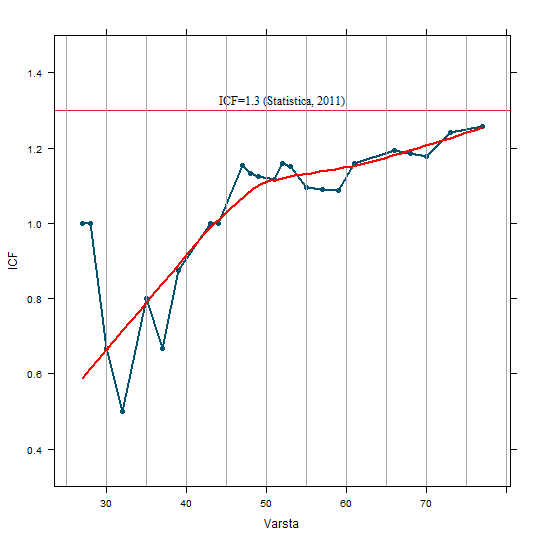
\includegraphics[width=0.8\linewidth]{incoNasteriICF}
    \caption{Variația ICF cu vârsta pacienților. Se observă convergența asimptotică către statistica națională (linia orizontala roșie) pe măsură ce sunt incluse persoanele trecute de perioada fertilă }
    \label{fig:incoNasteriICF}
  \end{figure}
  %
  
  Studiul a înregistrat și  date referitor la co-morbiditatea pacienților colectând date despre prezența următoarelor condiții medicale: bronșita cronică, diabet, sindrom Parkinson, mielită, spina bifida, depresie, fractură vertebrală, fractură de coloană sau \ac{AVC}. 24 de pacienți nu au raportat nici o condiție. Sumarul datelor este prezentat în tabelul \ref{tab:comoSumary}. 
  %
  \begin{table}[H]
    \centering
    \begin{tabular}{ |l| >{\centering\arraybackslash}p{1.4cm} | }
      \hline
      Condiție medicală & Număr \newline pacienți \\ \hline
      AVC & 7 \\ \hline
      DEPRESIE & 3 \\ \hline
      DIABET & 6 \\ \hline
      FRACTURĂ COLOANĂ & 2 \\ \hline
      FRACTURĂ VERTEBRALĂ & 1 \\ \hline
      MIELITĂ & 3 \\ \hline
      PARKINSON & 3 \\ \hline
      SPINA BIFIDA & 1 \\ \hline
    \end{tabular}
    \caption{Condiția medicală și numărul de persoane pentru fiecare}
    \label{tab:comoSumary}
  \end{table}
  %
  După cum se observă în Figura \ref{fig:incoComoCntBySex}, distribuția condițiilor medicale variază foarte mult în funcție de sexul pacientului, astfel încât pacienții de sex masculin raportează cele mai multe cazuri de co-morbiditate ($N_B=17$ vs $N_F=9$),  chiar dacă numărul lor total este mai mic în eșantion ($Total_B=19$ vs $Total_F=31$).
  \begin{figure}[H]
    \centering
    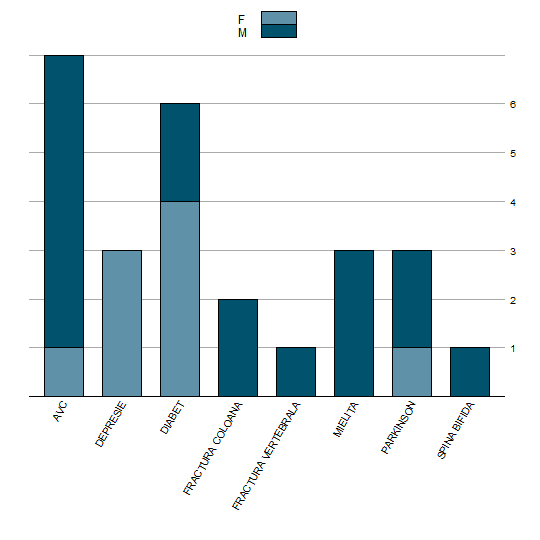
\includegraphics[width=0.8\linewidth]{incoComoCntBySex}
    \caption{Numărul de condiții medicale pentru fiecare sex. }
    \label{fig:incoComoCntBySex}
  \end{figure}
  %

\subsection{Efecte}
  Analiza datelor raportate de pacienți (atât cele subiective cât și cele obiective) a arătat o îmbunatățire consistentă a tuturor valorilor măsurate. Pentru rigurozitate am folosit testul t pentru a rejecta ipoteza nulă conform căreia nu exista nici o diferență după aplicarea tratamentului în parametrii măsurați. La toți parametrii, probabilitatea ca ipoteza nulă sa fie adevărată este $\ll 0.05$ ceea ce înseamnă ca efectul este real din punct de vedere statistic. Un sumar al parametrilor împreună cu intervale de încredere estimate de testul t este prezentat în tabela~\ref{tab:resTestSummary}.
  \begin{table}[H]
    \centering
    \begin{tabular}{|l|c|c|}
      \hline
       & $Pr(>|t|)$ & 95 \% CI \\   \hline
      I2D & 		$1.8e-22$ 	& $[ 6.50, 8.22 ]$ \\ \hline
      CEII & 		$4.4e-32$ 	& $[ 10.83, 12.49 ]$ \\ \hline
      CVDSU & $8.0e-30$ 	& $[ 3.96, 4.64 ]$ \\ \hline
      VAS & 		$1.8e-24$ 	& $[ 5.50, 6.78 ]$ \\ \hline
      USS & 		$7.2e-11$ 	& $[ 1.27, 2.09 ]$ \\ \hline
      FEFMP & $2.1e-25$ 	& $[ -2.31, -1.89 ]$ \\ \hline
    \end{tabular}
    \caption{Rezultatele testului t pentru parametrii măsurați} 
    \label{tab:resTestSummary}
  \end{table}
  %
  \begin{figure}[H]
    \centering
    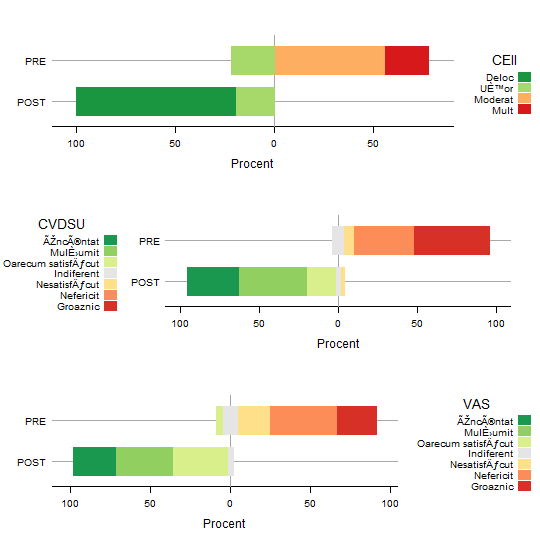
\includegraphics[width=0.8\linewidth]{incoResVariousStack}
    \caption{\ac{CEII},\ac{CVDSU},\ac{VAS} înainte și după tratament}
    \label{fig:incoResVariousStack}
  \end{figure}
  %
  În figura~\ref{fig:incoResVariousStack} se observă cum toți parametrii au migrat către valori considerate pozitive, aici reprezentate prin nuanțe de verde. 
  
  Un alt parametru care a înregistrat o îmbunatățire este \acf{USS}, care după cum se vede în figura~\ref{fig:incoResUSS} indica o scădere cu 71\% în agregat a numărului de prezentări la medic cauzate de probleme de incontinența.
  %
  \begin{figure}[H]
    \centering
    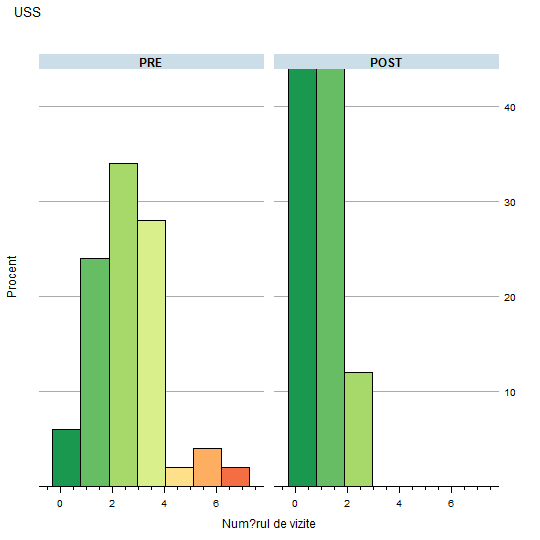
\includegraphics[width=0.8\linewidth]{incoResUSS}
    \caption{\acf{USS}}
    \label{fig:incoResUSS}
  \end{figure}
  %
  
  Datele obiective (numărul de episoade de incontinența pe 2 zile și \ac{FEFMP}) arată o îmbunatățire în urma tratamentului conform tabelului~\ref{tab:resTestSummary}. Pentru a evalua efectul tratamentului asupra \ac{FEFMP} am folosit modele lineare cu efecte fixe și testul ANOVA. Modelul selectat ca fiind cel mai bun folosind ANOVA este $y_{it} = X_{it}\mathbf{\beta}+\alpha_{i}+u_{it}$ unde $y_{it}$ este valoarea FEFMP pentru individul $i$ la momentul $t \in [PRE,POST]$, iar $X_{it}$ este vectorul de regresie $\left(\!\begin{array}{c}Trt\\group\end{array}\right)$. După cum se vede din tabela~\ref{tab:resFEFMPlm}, tratamentul este foarte semnificativ iar un grad mare de semnificație îl are și cauza incontinentei urinare, grupul care suferă de \ac{IUI} având un răspuns mai prost la tratament fata de cei ce suferă de \ac{IUE} dar față de efectul tratamentului, influența cauzei este de 5 ori mai slabă.
  Pentru I2D, am inclus în modelul linear și un termen legat de numărul de nașteri, dar rezultatele nu indică semnificație statistică nici pentru cauza incontinenței și nici pentru numărul de nașteri. Mai precis, numărul de nașteri este corelat slab ($p=0.17$ insuficient pentru pragul de  relevanță statistică ales de $p<0.05$) cu datele conform tabelului~ \ref{tab:resI2Dlm}.
  %
  \begin{table}[H]
		\centering
		\begin{tabular}{rrrrr}
			\hline
			& Est. & $\sigma~~~$ & Pr($>|t|$) \\ \hline
			(Intercept) & 2.21 & 14.35 & 0.000 \\ 
			TrtPOST & 2.10  & 11.81 & 0.000 \\ 
			groupIUI & -0.38 & -2.14 & 0.035 \\ \hline
		\end{tabular}
		\caption{Rezultatele modelului linear pentru FEFMP} 
		\label{tab:resFEFMPlm}
	\end{table}
  
	\begin{table}[H]
		\centering
		\begin{tabular}{rrrrr}
			\hline
			& Est. & $\sigma~~~$ & Pr($>|t|$) \\ \hline
			(Intercept) & 7.99 & 0.71 & 0.00 \\ 
			TrtPOST & -7.06 & 0.69 & 0.00 \\ 
			Nașteri & 0.57 & 0.41 & 0.17 \\
			groupIUI & 0.67 & 0.88 & 0.44 \\ \hline
		\end{tabular}
		\caption{Rezultatele modelului linear pentru I2D} 
		\label{tab:resI2Dlm}
	\end{table}
  %
\subsubsection{Analiza influenței tipului de incontinență}
 După cum a fost menționat în secțiunea~\nameref{rezPop}, la studiu au participat un număr egal ($n_1=n_2=25$) de pacienți care suferă de \ac{IUE} și de \ac{IUI}.ÎIntre aceste 2 grupuri există diferențe atât în parametrii populației (vârsta, sex, co-morbiditate, etc.) precum și în rezultatele după aplicarea tratamentului. Grupul pacienților care suferă de \ac{IUE} este compus exclusiv de paciente de sex feminin cu vârste cuprinse între 28 și 77 de ani, iar grupul care suferă de \ac{IUI} este compus preponderent din bărbați (76\%, n=19) cu vârste cuprinse între 30 și 83 ani, iar femeile (24\%, n=6) au vârstele între 27 și 77 ani. După cum am arătat anterior (vezi figura~\ref{fig:incoComoCntBySex}), bărbații au de asemenea cel mai mare număr de probleme medicale.
Efectele tratamentului înregistrate prin chestionare sunt influențate de tipul de incontinență care se dovedește a avea un efect semnificativ statistic ($p<0.05$) doar în 2 cazuri: \ac{CVDSU} și \ac{VAS} înainte de tratament și un efect nesemnificativ în \ac{FEFMP} după tratament. Valorile $p$ pentru corelarea dintre toate datele colectate pe scale Likert și grup, înainte și după tratament se găsesc în tabela~\ref{tab:resFisherGroup}. 
 %
 \begin{table}[H]
	\centering
	\begin{tabular}{|l|c|c|} \hline
	   																	& $p$ PRE 													& $p$ POST \\ \hline
		CEII 														& 0.23151 													& 0.53621 \\ \hline
		\textcolor{green}{CVDSU} 	& \textcolor{green}{0.03888} 	& 0.60262 \\ \hline
		\textcolor{green}{VAS} 			& \textcolor{green}{0.04250} 	& 0.11972 \\ \hline
		IGPI 														& NA 																&  0.33212 \\ \hline
		USS 															& 0.28003 													& 0.30178 \\ \hline
		\textcolor{yellow}{FEFMP} 	& 0.15156 													& \textcolor{yellow}{0.08047} \\ \hline
	\end{tabular}
	\caption{Rezultatele testelor Fisher pentru asocierea dintre valoarea înregistrata și grup} 
	\label{tab:resFisherGroup}
\end{table}
%
Pentru a aprecia magnitudinea efectelor tratamentului în funcție de apartenență la grup am construit un model linear pentru valorile \ac{CVDSU}, \ac{VAS} și \ac{FEFMP}. Figura~\ref{fig:incoResRegGrp} arată o îmbunatățire mai puternică în privința acestor 2 valori raportate pentru grupa pacienților care suferă de \ac{IUI} ($\beta=-4.68, t(48)=0.6258, p\ll0.01$) față de grupa pacienților care suferă de \ac{IUE} ($\beta=-3.92, t(48)=1.136, p\ll0.01$) (pantele liniilor de regresie sunt mai mari în valori absolute pentru \ac{IUI}, iar semnul negativ indică o scădere a valorilor după aplicarea tratamentului). Aceeași analiza a fost repetată pentru \ac{FEFMP} (vezi figura~\ref{fig:incoResRegFEFMP}) care indică o îmbunatățire mai mare pentru pacienții care suferă de \ac{IUE} ($\beta=2.20, t(48)=0.831, p\ll0.01$) față de cei care suferă de \ac{IUI} ($\beta=2.00, t(48)=0.950, p\ll0.01$) însă această observație nu este semnificativă din punct de vedere statistic ($p=0.08047>0.05$).
  %
  \begin{figure}[H]
    \centering
    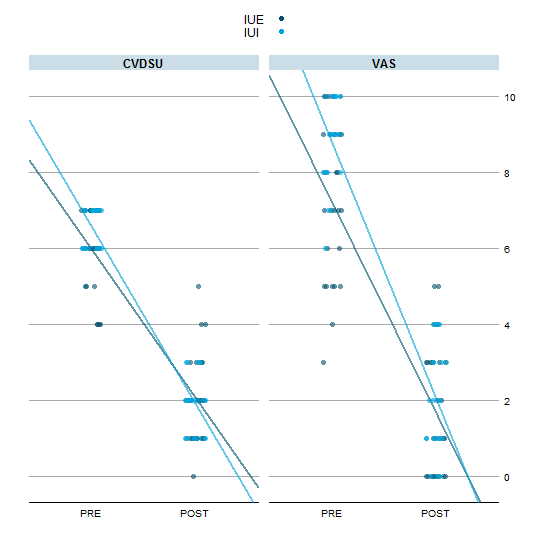
\includegraphics[width=0.8\linewidth]{incoResRegGrp}
    \caption{Evoluția \acf{CVDSU} și \acf{VAS} pentru cele 2 grupe}
    \label{fig:incoResRegGrp}
  \end{figure}
  %
  \begin{figure}[H]
    \centering
    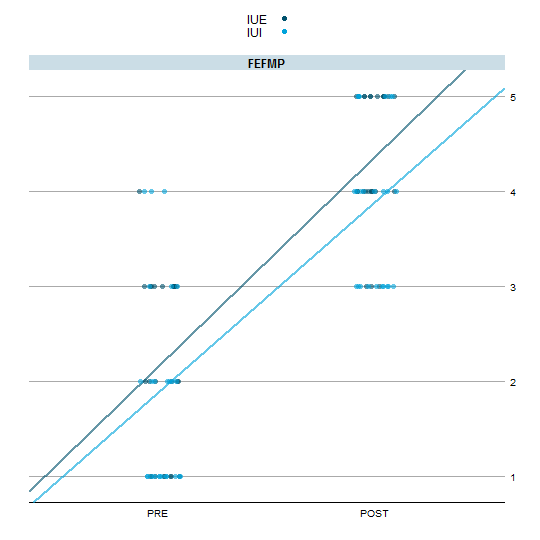
\includegraphics[width=0.8\linewidth]{incoResRegFEFMP}
    \caption{Evoluția \acf{FEFMP}}
    \label{fig:incoResRegFEFMP}
  \end{figure}
  %

 %%%% 
\Section{Concluzii}
 Tratamentul aplicat acestor pacienți îmbunătățește semnificativ toate valorile măsurate, atât cele subiective cât și cele obiective, reduce cu 87\% ($\approx2\sigma$) numărul de episoade de incontinență măsurate pe parcursul a 2 zile și mărește cu 50\% ($\approx2\sigma$) forța musculaturii perineale măsurată conform \acf{FEFMP}. Aceste efecte sunt robuste indiferent dacă pacienții suferă de \acf{IUE} sau \acf{IUI}. Între aceste 2 grupuri de pacienți sunt diferențe semnificative de sex, vârsta, co-morbidități și în cazul unor evaluări subiective (\acf{CVDSU} și \acf{VAS}). Efectele tratamentului diferă semnificativ statistic între aceste 2 grupuri doar în cazul datelor pentru \ac{CEII}, \ac{CVDSU} unde indică o îmbunatățire mai pronunțată pentru pacienții care suferă de \ac{IUI} și pentru \ac{FEFMP} unde indică o îmbunatățire mai pronunțată pentru cei ce suferă de \ac{IUE}. Nu trebuie pierdut din vedere ca aceste corelații (mai ales pentru evaluările subiective unde pot exista influene culturale profunde) se pot datora unor parametrii care nu au fost măsurați în acest studiu chiar dacă au ieșit în evidență la compararea celor 2 grupuri de pacienți -- grupurile sunt suficient de ne-omogene pentru a intui că pot exista alți factori care sa influențeze valorile măsurate în afara faptului că un pacient suferă de \ac{IUI} și nu de \ac{IUE}.  
 
 Impresiile pacienților despre efectele tratamentului, colectate la sfârșitul studiului clinic coincid cu rezultatele noastre, mai mult de 70\% ($n=39$) raportând că se simt mai bine sau mult mai bine față de situația anterioară.
  %
  \begin{figure}[H]
    \centering
    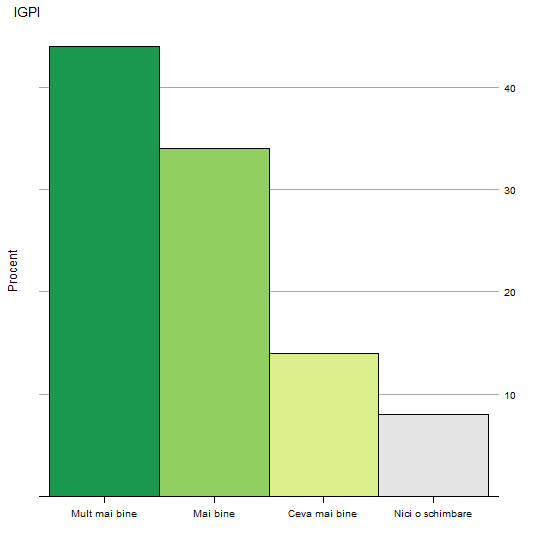
\includegraphics[width=0.8\linewidth]{incoResIGPI}
    \caption{\acf{IGPI} la sfârșitul tratamentului}
    \label{fig:incoResIGPI}
  \end{figure}
  %
 
   
  \closeopenmulticols
  
  \bibliographystyle{plainnat}\bibliography{incoStudy}
  
  \section*{Glosar}
  \begin{acronym}[LUTS]
    \acro{IU}{Incontinența Urinară}
    \acro{IUI}{Incontinența Urinară prin Imperiozitate}
    \acro{IUE}{Incontinența Urinară de Efort}
    \acro{IUM}{Incontinența Urinară Mixtă}
    \acro{LUTS}{Lower Urinary Tract Symptoms}
    \acro{TOT}{Trans Obturator vaginal Tape} 
    \acro{TVT}{Tension free Vaginal Tape}
    \acro{SEP}{Stimulare Electrica Periferica}
    \acro{BMI}{Body-Mass Index}
    \acro{KS}{Kolmogorov–Smirnov}
    \acro{ICF}{Indicatorul Conjunctural de Fertilitate}
    \acro{AVC}{Accident vascular cerebral}
    \acro{CEII}{Chestionar de Evaluare a Impactului Incontinentei}
    \acro{CVDSU}{Calitatea Vieții Datorată Simptomelor Urinare}
    \acro{VAS}{Scala Vizual Analogică pentru evaluarea gradului de îmbunătățire a calității vieții}
    \acro{FEFMP}{Fisa de Evaluare a Forței Musculaturii Perineale}
    \acro{IGPI}{Impresia Globala a Pacientului de Îmbunătățire}
    \acro{USS}{Utilizarea Serviciilor De Sănătate}
  \end{acronym}
 
 \listoffigures
 \listoftables
   
\end{document}
